\documentclass{crebsshr}

%%%%%%%%% Journal Info -- DO NOT CHANGE %%%%%%%%%
\setcounter{page}{1}
\setcounter{secnumdepth}{4}
\renewcommand\thisnumber{x}
\renewcommand\thisyear {202x}
\renewcommand\thisvolume{x}
\renewcommand\datereceived{xxxx xx, 202x}
\renewcommand\dateaccepted{xxxx xx, 202x}
\renewcommand\dateavailable{xxxx xx, 202x}
\renewcommand\doinumber{10.62366/crebss.202x.x.00x}
\renewcommand\type{XXX XXX}
\renewcommand\JEL{XXX, XXX}
%%%%%%%%% End Journal Info   %%%%%%%%%

\usepackage{graphicx}
\usepackage{amsmath}
\usepackage{fontawesome}
\usepackage{hyperref}
\usepackage{xcolor}
\usepackage{float}  % For [H] placement
\usepackage{booktabs}  % For professional tables
\usepackage{subcaption}  % For subfigures
\usepackage{geometry}  % Adjust margins if needed

% Custom commands from the blueprint
\newcommand{\affilnum}[1]{\textsuperscript{#1}}

% Begin document
\begin{document}

% The title, author, abstract, etc., will be inserted by R Markdown

\subsection{R Markdown}\label{r-markdown}

This is an R Markdown document. Markdown is a simple formatting syntax
for authoring HTML, PDF, and MS Word documents. For more details on
using R Markdown see \url{http://rmarkdown.rstudio.com}.

When you click the \textbf{Knit} button a document will be generated
that includes both content as well as the output of any embedded R code
chunks within the document. You can embed an R code chunk like this:

\begin{Shaded}
\begin{Highlighting}[]
\FunctionTok{summary}\NormalTok{(cars)}
\end{Highlighting}
\end{Shaded}

\begin{verbatim}
##      speed           dist       
##  Min.   : 4.0   Min.   :  2.00  
##  1st Qu.:12.0   1st Qu.: 26.00  
##  Median :15.0   Median : 36.00  
##  Mean   :15.4   Mean   : 42.98  
##  3rd Qu.:19.0   3rd Qu.: 56.00  
##  Max.   :25.0   Max.   :120.00
\end{verbatim}

\subsection{Including Plots}\label{including-plots}

You can also embed plots, for example:

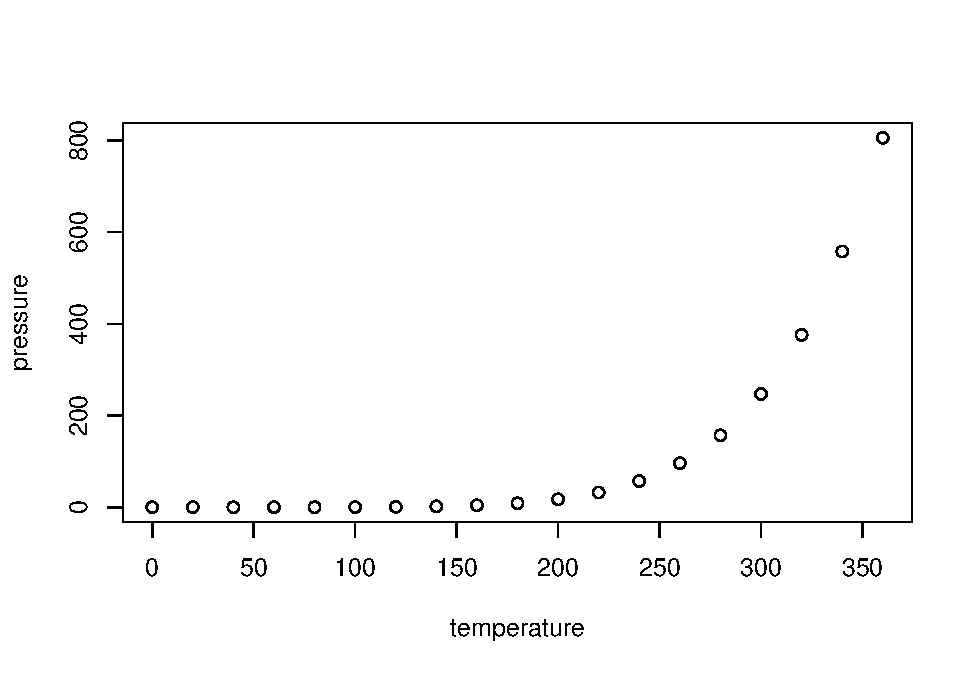
\includegraphics{plroba_latex_files/figure-latex/pressure-1.pdf}

Note that the \texttt{echo\ =\ FALSE} parameter was added to the code
chunk to prevent printing of the R code that generated the plot.

% Bibliography (if using BibTeX)
\bibliographystyle{plain}
\bibliography{references}

\end{document}
